\section{Resultados}

{
\setbeamercolor{background canvas}{bg=beamer@blendedblue!30}
\begin{frame}
  % frame contents here
    \centering
  \Huge
  Resultados
\end{frame}
}

\begin{frame}
\frametitle{\(v_a\) en función del tiempo}
\begin{columns}
    \begin{column}{0.6\textwidth}
      \begin{center}
        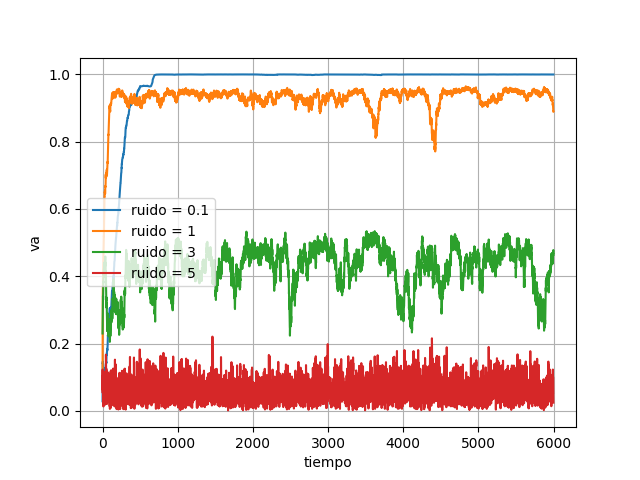
\includegraphics[width=\textwidth]{images/va-vs-tiempo-noise.png} % Replace with your image file 
      \end{center}
    \end{column}
    \begin{column}{0.4\textwidth}
                \footnotesize
       \begin{center}
                \begin{itemize}
        \item \(L = 10\)
        \item \(N = 400\)
        \end{itemize}
       \end{center}
    \end{column}
\end{columns}
        \begin{itemize}
        \item \(\eta \in \{3,5\}\): \(v_a\) no se estabiliza.
        \item \(\eta = 0.1\): \(v_a\) se estabiliza desde \(t \approx 700\).
                \item \(\eta = 1\): \(v_a\) se estabiliza desde \(t \approx 4500\).
        \end{itemize}
\end{frame}

\begin{frame}
\frametitle{\(v_a\) en función del tiempo}
\begin{columns}
    \begin{column}{0.6\textwidth}
      \begin{center}
        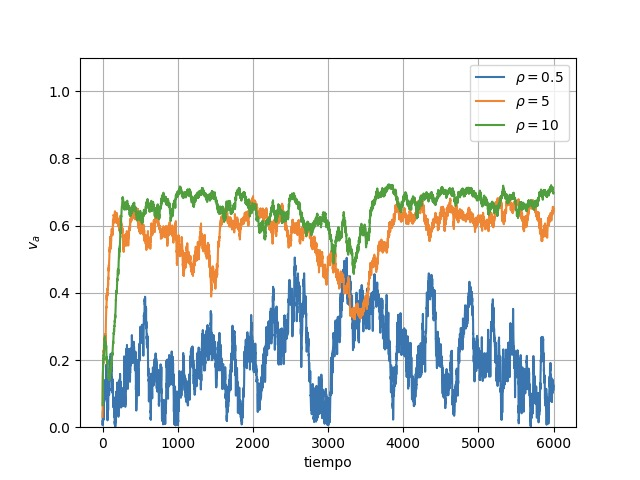
\includegraphics[width=\textwidth]{images/va-vs-tiempo-density.jpeg} % Replace with your image file 
      \end{center}
    \end{column}
    \begin{column}{0.4\textwidth}
\begin{center}
            \footnotesize
        \begin{itemize}
        \item \(L = 20\)
        \item \(\eta = 2.5\)
        \end{itemize}
\end{center}
    \end{column}
\end{columns}
        \begin{itemize}
        \item \(\rho \in \{5,10\}\): \(v_a\) se estabiliza desde \(t \approx 4000\)
        \item \(\rho = 0.5\): \(v_a\) no se estabiliza.
        \end{itemize}
\end{frame}

\begin{frame}
\frametitle{Cálculo de \(v_a\)}
Se decide utilizar el siguiente método:
 \begin{itemize}
        \item Si la variación de \(v_a\) en 10 iteraciones consecutivas es \(< 0.01\), se toma ese promedio.
        \item Si al llegar a la iteración 5000 no se cumplió la condición anterior, se calcula \(v_a\) como el promedio de las iteraciones 5001 a 6000.   
        \end{itemize}
\end{frame}
\begin{frame}
\frametitle{\(v_a\) en función del ruido}
\begin{columns}
    \begin{column}{0.6\textwidth}
      \begin{center}
        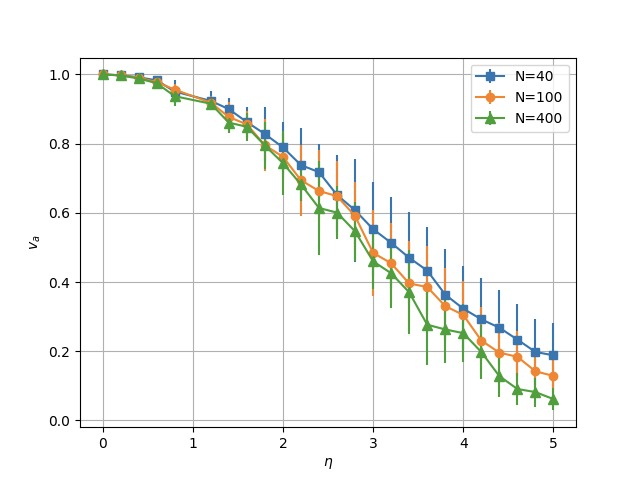
\includegraphics[width=\textwidth]{images/va-vs-ruido.jpeg} % Replace with your image file 
      \end{center}
    \end{column}
    \begin{column}{0.4\textwidth}
                \footnotesize
\begin{center}
            \begin{itemize}
        \item \(\rho = 4\)
        \end{itemize}
\end{center}
    \end{column}
\end{columns}
\end{frame}
\begin{frame}
\frametitle{\(v_a\) en función de la densidad}
\begin{columns}
    \begin{column}{0.6\textwidth}
      \begin{center}
        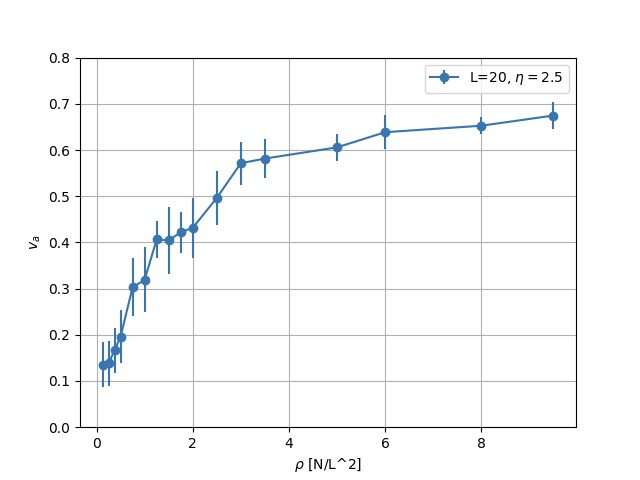
\includegraphics[width=\textwidth]{images/va-vs-density.jpeg} % Replace with your image file 
      \end{center}
    \end{column}
    \begin{column}{0.4\textwidth}
                \footnotesize
    \begin{center}
                \begin{itemize}
        \item \(\eta = 2.5\)
        \item \(  L = 20\)
        \end{itemize}
    \end{center}
    \end{column}
\end{columns}
\end{frame}